\chapter{OWL}
\label{chap:owl}

Im vorherigen Kapitel wurden Voraussetzungen geschaffen um die eigentliche Ontologiesprache, OWL zu analysieren. In diesem Kapitel, auf~\cite{w3owl} basierend, wird OWL näher betrachtet.

Bei OWL (Web Ontology Language) handelt es sich um eine Ontologiesprache für das semantische Web. Mit dieser Sprache können Ontologien beschrieben werden.~\cite{cambSemOWL} Wie RDF wurde auch OWL nicht nur für die Anzeige sondern auch für die Verarbeitung von Informationen entwickelt.

Durch zusätzliches Vokabular, wie Beziehungen zwischen Klassen, erweiterter formaler Semantik hat der Benutzer mehr Möglichkeiten als bei RDF/XML oder auch XML.\@

\section{OWL Syntax}
\label{sec:owl_owl_syntax}
Für OWL stehen verschiedene Schreibweisen zur Verfügung, welche für verschiedene Anwendungen definiert wurden:
\begin{itemize}
	\item \textit{RDF/XML Syntax für OWL}

        Entspricht der RDF/XML Syntax mit einer spezifischen Übersetzung für OWL-Konstrukte. Es ist die einzige Syntax, welche von allen OWL2-Werkzeugen unterstützt wird (OWL2 ist die letzte Version von OWL).
	\item \textit{OWL/XML Syntax}

        XML Syntax für OWL.\@
	\item \textit{Functional-Style Syntax}

        Sie dient der Vereinfachung der ursprünglichen Spezifikation. Sie unterstützt Grundlagen zur Implementation von OWL2 durch APIs und Reasoners.
	\item \textit{Turtle Syntax}

        Bei der Turtle Syntax handelt es sich um eine textuelle Syntax, welche die Beschreibung eines RDF-Graphen in kompakter und natürlicher Form erlaubt.

	\item \textit{Manchester Syntax}

        Vereinfacht das Lesen und Verstehen für Leser ohne Kenntnisse der Prädikatenlogik.
\end{itemize}

Anmerkung: Es existieren Werkzeuge, welche eine Übersetzung zwischen den verschiedenen Schreibweisen zulassen.

Bei OWL handelt es sich nicht um eine Schemasprache. Im Gegensatz zu XML beschreibt OWL nicht, wie ein Dokument aufgebaut sein muss. So kann das Vorhandensein eines bestimmten Elementes nicht vorgeschrieben werden.

\begin{lstlisting}[caption={Beispiel der Turtle Syntax\protect\footnotemark}]
    <#green-goblin>
        rel:enemyOf <#spiderman> ;
        a foaf:Person ;    # in the context of the Marvel universe
        foaf:name "Green Goblin".
\end{lstlisting}
\footnotetext{Beispiel von \url{http://www.w3.org/TR/turtle}}

\section{Wissen modellieren}
\label{sec:owl_owl_wissenModellieren}
Bei OWL handelt ist eine wissensbasierte Repräsentationssprache. Sie widerspiegelt das Wissen einer spezifischen Domäne. Dabei wird versucht eine Domäne mittels OWL so abzubilden, dass sie Teilen des menschlichen Wissens entspricht. Eine Möglichkeit alle Aspekte des menschlichen Wissens abzubilden besteht aber nicht. Trotzdem kann OWL als potente Modellierungssprache bezeichnet werden. Das Ergebnis einer solchen Modellierung ist eine Ontologie, wie bereits ausgeführt.

Für die Wissensabbildung über OWL werden grundlegende Konzepte wie Axiome, Entitäten und Ausdrücke (Expressions) benutzt.


\begin{itemize}
    \item \textit{Axiom}

        Grundlegende Aussage.

        Grundaussagen  oder Basispropositionen wie ``Abenteuerreisen sind Reisen'' werden in OWL Axiome genannt. Es handelt sich  um ``Teile des Wissens'', welche je nach Sachlage wahr oder falsch sein können. Dies ist ein essentieller Unterschied zu Entitäten und Ausdrücken.

    \item \textit{Entitäten}

        Elemente, welche konkrete Objekte aus der realen Welt abbilden.

        Grundbestandteile einer Aussage werden Entitäten genannt, zum Beispiel Objekte wie ``Abenteuerreise'' und ``Reise'' oder Beziehungen wie ``sind''.\\
        Konkrete Objekte werden dabei als Individuen (Individuals), Kategorien (für Individuen) als Klassen und Beziehungen (zwischen Individuen) als Eigenschaften (Properties) bezeichnet.\\
        Beziehungen werden unterteilt in Relationen zwischen zwei Individuen (ObjectProperties), spezifischen Datenwerten von Individuen (DataProperties) und zusätzliche Informationen zu einem Objekt (AnnotationProperties).

	\item \textit{Expression (Ausdruck)}

        Ausdrücke sind Kombinationen aus Entitiäten. Sie ermöglichen den Aufbau von komplexen Beschreibungen.

        Entitäten, wie z.B. Klassen, können mit Hilfe eines Konstruktors kombiniert werden. Beispiel: ``Abenteuerreise'' und ``Reise''. Diese Kombination wird als ClassExpression abgebildet und ist eine neue Entität.

        Ausdrücke (Ausdruckssprache) sind für Klassen sehr vielfältig, hingegen nicht für Eigenschaften.

        \begin{lstlisting}[caption={Beispiel eines Ausdrucks: Zwei Klassen bedeuten das Gleiche}]
            EquivalentClasses(
                :Restaurant
                :Gaststätte
            )
        \end{lstlisting}

\end{itemize}


\section{Die wichtigsten Elemente von OWL}
\label{sec:owlRdf_owl_wichtigsteElemente}

\subsection{Klassen, Subklassen und Individuen}
\label{sec:owlRdf_owl_wissenModellieren_wichtigsteElemente_Classen}

\textbf{Klassen} werden dazu verwendet, um Individuen mit Gemeinsamkeiten zu gruppieren. Klassen stellen daher eine Menge von Individuen dar. Für die Abbildung der menschlichen Denkweise, werden in der Modellierung Klassen verwendet, beispielsweise Reisen oder Abenteuerreisen.

Beispiel: \textit{Abenteuerreise} ist (nach unserer Definition) eine Klasse.

\begin{lstlisting}[caption={Beispiel einer Klasse: Ausflüge}]
    <!-- http://www.semanticweb.org/sosterwalder/ontologies/2014/10/reiseplaner#Ausflug -->
    <owl:Class rdf:about="&reiseplaner;Ausflug"/>
\end{lstlisting}

\textbf{Subklassen}
Im obigen Abschnitt wurden die Klassen Reise sowie Abenteuerreise eingeführt. Der menschliche Leser weiss intuitiv, dass eine Abenteuerreise auch eine Reiseform ist.

In OWL stehen diese beiden Klassen jedoch nicht in Beziehung. Es handelt sich um zwei unterschiedliche Klassen mit unterschiedlichen Bezeichnungen. Um die Schlussfolgerung, eine Abenteuerreise ist auch eine Reise, zu erreichen, muss dies definiert werden. In OWL geschieht dies mit dem Subklassen-Axiom $subClassOf$.

Beispiel: \textit{Landgasthaus} ist (nach unserer Definition) Subklasse von \textit{Restaurant}.

\begin{lstlisting}[caption={Beispiel einer Subklasse}]
    <!-- http://www.semanticweb.org/sosterwalder/ontologies/2014/10/reiseplaner#Landgasthaus -->
    <owl:Class rdf:about="&reiseplaner;Landgasthaus">
        <rdfs:subClassOf rdf:resource="&reiseplaner;Restaurant"/>
    </owl:Class>
\end{lstlisting}
Nicht nur zur Darstellung von Abhängigkeiten werden Subklassen verwendet, sondern auch zur Modellierung von Klassenhierarchien. Mittels Subklassen werden allgemeine Beziehungen der Klassen abgebildet, so zum Beispiel die Relation ``ein Landgasthaus ist ein Restaurant.''

Bei \textbf{Individuen} handelt es sich um \textit{Instanzen von Klassen}. Ein Individuum ist Mitglied der Menge einer Klasse und bildet daher deren Konzept ab. Individuuen können gleichzeitig Mitglied von mehreren Klassen sein.

Beispiel: \textit{Seilpark Balmberg} ist (nach unserer Definition) ein Individuum der Klasse \textit{Ausflug}. 

\begin{lstlisting}[caption={Beispiel eines Individuums}]
    <!-- http://www.semanticweb.org/sosterwalder/ontologies/2014/10/reiseplaner#Seilpark -->
    <owl:NamedIndividual rdf:about="&reiseplaner;Seilpark">
        <rdf:type rdf:resource="&reiseplaner;Ausflug"/>
        <reiseplaner:alter rdf:datatype="&xsd;integer">6</reiseplaner:alter>
        <reiseplaner:erfordert>mut</reiseplaner:erfordert>
        <reiseplaner:erfordert>geschicklichkeit</reiseplaner:erfordert>
        <reiseplaner:url>http://www.seilpark-balmberg.ch/</reiseplaner:url>
        <reiseplaner:hatStandort rdf:resource="&reiseplaner;Balmberg"/>
    </owl:NamedIndividual>
\end{lstlisting}

\newpage

Mittels der \textit{owl:sameAs-Relation} kann ausgedrückt werden, dass es sich bei zwei oder mehreren Individuen um die gleichen Individuen handelt.

\begin{lstlisting}[caption={Beispiel einer Gleichstellung von Individuen: Seilpark und Seilpark-Balmberg sind das gleiche Individuum}]
    <!-- http://www.semanticweb.org/sosterwalder/ontologies/2014/10/reiseplaner#Seilpark -->
    <owl:NamedIndividual rdf:about="&reiseplaner;Seilpark">
        <rdf:type rdf:resource="&reiseplaner;Ausflug"/>
        ...
        <owl:sameAs rdf:resource="&reiseplaner;Seilpark_Balmberg"/>
    </owl:NamedIndividual>
\end{lstlisting}


Durch die \textit{owl:AllDifferent-Relation} kann das Gegenteil ausgesagt werden:  Zwei oder mehrere Individuen sind nicht die gleichen Individuen.

\begin{lstlisting}[caption={Beispiel einer Differenzierung von Individuen: Seilpark ist nicht das gleiche Individuum wie Seilpark-Pilatus}]
    <rdf:Description>
        <rdf:type rdf:resource="&owl;AllDifferent"/>
        <owl:distinctMembers rdf:parseType="Collection">
            <rdf:Description rdf:about="&reiseplaner;Seilpark"/>
            <rdf:Description rdf:about="&reiseplaner;Seilpark_Pilatus"/>
        </owl:distinctMembers>
    </rdf:Description>

\end{lstlisting}

\subsubsection{Eigenschaften}
\label{subsubsec:owlRdf_owl_wissenModellieren_wichtigsteElemente_Propertys}

\textbf{Objekt-Eigenschaften (ObjectProperties)}

Objekt-Eigenschaften beschreibt die Beziehung zwischen zwei Individuen.

\begin{lstlisting}[caption={Beispiel einer Objekteigenschaft \textit{hatOrt} und deren Anwendung}]
    <owl:ObjectProperty rdf:about="&reiseplaner;hatOrt">
        <rdfs:range rdf:resource="&reiseplaner;Ort"/>
        <rdfs:domain rdf:resource="&reiseplaner;Region"/>
    </owl:ObjectProperty>
    ...
    
    <owl:Thing rdf:about="&reiseplaner;Bern">
        <rdf:type rdf:resource="&owl;NamedIndividual"/>
        <reiseplaner:distanzZuAusgangpunkt rdf:datatype="&xsd;integer">0</reiseplaner:distanzZuAusgangpunkt>
        <reiseplaner:hatOrt rdf:resource="&reiseplaner;Bern"/>
        <reiseplaner:hatOrt rdf:resource="&reiseplaner;Ersigen"/>
    </owl:Thing>
\end{lstlisting}

Durch Auswahl von Klassen kann eingeschränkt werden, auf welche Individuen eine Objekt-Eigenschaft angwendet werden darf. Dies gilt sowohl für die Quelle einer Beziehung (Domäne, Domains) als auch für das Ziel einer Beziehung (Wertebereich, Ranges).


\begin{lstlisting}[caption={Beispiel von Einschränkungen der Objekteigenschaft \textit{hatRegion}}]
    <!-- http://www.semanticweb.org/sosterwalder/ontologies/2014/10/reiseplaner#hatRegion -->
    <owl:ObjectProperty rdf:about="&reiseplaner;hatRegion">
        <rdfs:domain rdf:resource="&reiseplaner;Land"/>
        <rdfs:range rdf:resource="&reiseplaner;Region"/>
    </owl:ObjectProperty>
\end{lstlisting}

\textbf{Subeigenschaften}

Analog zu Subklassen lassen sich Untereigenschaften (Subproperties) definieren.

\begin{lstlisting}[caption={Beispiel der Objekteigenschaft \textit{hatGemeinde} als Subeigenschaft von \textit{hatRegion}}]
    <!-- http://www.semanticweb.org/sosterwalder/ontologies/2014/10/reiseplaner#hatGemeinde -->
    <owl:ObjectProperty rdf:about="&reiseplaner;hatGemeinde">
        <rdfs:subPropertyOf rdf:resource="&reiseplaner;hatRegion"/>
    </owl:ObjectProperty>
\end{lstlisting}

\textbf{Datentypen-Eigenschaften (DataProperties)}

Datentypen-Eigenschaften definieren und beschreiben einen spezifischen Datenwert eines Individuums. Dies können beispielsweise das Alter oder die Grösse einer Person sein. Datentypen-Eigenschaft können frei definiert werden und, bei Bedarf, an vordefinierte Wertetypen gebunden werden. Eine Auflistung vordefinierter Wertetypen findet sich unter der Webseite~\href{http://www.w3.org/TR/owl2-syntax/\#Datatype_Maps}{w3.org}\footnote{\url{http://www.w3.org/TR/owl2-syntax/\#Datatype_Maps}}.

\begin{lstlisting}[caption={Beispiel der Datentypen-Eigenschaft \textit{anzahlTeilnehmer} und deren Anwendung bei einem Individuum}]
    <!-- http://www.semanticweb.org/sosterwalder/ontologies/2014/10/reiseplaner#anzahlTeilnehmer -->
    <owl:DatatypeProperty rdf:about="&reiseplaner;anzahlTeilnehmer">
        <rdfs:range rdf:resource="&xsd;integer"/>
        <rdfs:subPropertyOf rdf:resource="&owl;topDataProperty"/>
    </owl:DatatypeProperty>
    ...
    <!-- http://www.semanticweb.org/sosterwalder/ontologies/2014/10/reiseplaner#AdventureRooms -->
    <owl:NamedIndividual rdf:about="&reiseplaner;AdventureRooms">
        ...
        <reiseplaner:anzahlTeilnehmer rdf:datatype="&xsd;integer">12</reiseplaner:anzahlTeilnehmer>
        ...
    </owl:NamedIndividual>
\end{lstlisting}

\newpage

\section{Ontologien}
\label{sec:owl_owl_Ontologien}

Wissensdomänen zu einem Thema werden in Ontologien abgebildet. Diese können für verschiedenen Anwendungen genutzt werden.

\begin{lstlisting}[caption={Beispiel einer Definition einer Ontologie}]
    <owl:Ontology rdf:about="http://www.semanticweb.org/sosterwalder/ontologies/2014/10/reiseplaner"/>
\end{lstlisting}

Ontologien werden als OWL-Dokumente abgespeichert. Dabei steht es dem Autor frei, sie im Internet zur Verfügung zu stellen.
Namespaces können zusätzlich beim Schreiben einer Ontologie verwendet werden. Sie dienen der Unterscheidbarkeit von Ontologien. Beispiel: ``\textit{meineOntologie\#}''. Um eine Onotlogie anhand deren Namespace benutzten zu können, wird ein Präfix definiert und dieser einer Ontologie zugewiesen. Beispiel: ``\textit{PREFIX hallo: <meineOntologie\#>}''. Somit können die Elemente der Ontologie mit dem Präfix angesprochen werden. Beispiel: ``\textit{hallo:objekt1DerOntologie}''.

Informationen aus einer beliebigen Ontologie können in einer anderen verwendet werden. Dafür ist ein Import der Ontologie nötig.

\begin{lstlisting}[caption={Beispiel eines Importes einer Ontologie}]
    <owl:Ontology rdf:about="http://example.com/owl/families\">
      <owl:imports rdf:resource="http://example.org/otherOntologies/families.owl" />
    </owl:Ontology>
\end{lstlisting}


Um bei der Verwendung von Objekten aus anderen Ontologien eine Umbenennung zu umgehen, kann direkt auf das entsprechende Objekt referenziert werden.

\begin{lstlisting}[caption={Beispiel einer Referenzierung auf ein Objekt einer externen Ontologie}]
    <owl:DatatypeProperty rdf:about="hasAge">
      <owl:equivalentProperty rdf:resource="\&otherOnt;age"/>
    </owl:DatatypeProperty>
\end{lstlisting}

\section{OWL Untersprachen}
\label{sec:owl_owl_Untersprachen}
OWL ist in drei Untersprachen aufgeteilt: OWL Lite, OWL DL und OWL full. Jede dieser Sprachen wurde für verschiedene Anwendergruppen entwickelt.

Die Version 2 von OWL unterscheidet zusätzlich zwischen OWL2 QL, OWL2 EL und OWL2 RL. Dies sind weitere Unterklassen von OWL2 DL, welche ihrerseits wiederum eine Untersprache von OWL2 full ist.

Genauere Informationen über die einzelnen Untersprachen finden sich unter der Webseite~\href{http://www.w3.org/TR/2004/REC-owl-features-20040210/\#s1.3}{w3.org/TR/2004/REC-owl-features}\footnote{\url{http://www.w3.org/TR/2004/REC-owl-features-20040210/\#s1.3}}, über OWL2-Profile unter~\href{http://www.w3.org/TR/owl2-profiles/}{w3.org/TR/owl2-profiles}\footnote{\url{http://www.w3.org/TR/owl2-profiles/}}

Die drei wichtigsten Unterklassen werden nachfolgend kurz vorgestellt.
\begin{itemize}
    \item \textit{OWL Lite}

        Bietet primär eine Hierarchie zur Klassifikation sowie einfache Bedingungen, so wird zwar z.B.\ Kardinalität geboten, jedoch nur mit den Werten 0 und 1.~\cite{w3owl}

    \item{\textit{OWL DL}}

        Bietet das Maximum an Ausdrucksmöglichkeiten unter Einhaltung der Vollständigkeit (alle Folgebeziehungen werden berücksichtigt und miteinbezogen) und der Entscheidbarkeit (alle Berechnungen enden nach endlicher Zeit).~\cite{w3owl}

    \item{\textit{OWL full}}

        Bietet das Maximum an Ausdrucksmöglichkeiten und die syntaktische Freiheit von RDF aber ohne Garantien betreffend Vollständigkeit und Entscheidbarkeit.''~\cite{w3owl}

\end{itemize}

\section{OWL-Werkzeuge}
\label{sec:owl_owl_OwlTools}
Typischerweise unterscheidet man zwischen zwei Arten von Ontologiewerkzeugen, einem Editor und einem Reasoner. Der Editor ermöglicht das Erstellen und Ändern von Ontologien. Der Reasoner leitet logische Folgerungen aus dem bestehenden Wissen ab.

\noindent\rule[1ex]{\textwidth}{1pt}
\begin{wrapfigure}[5]{l}{0.1\textwidth}
    \vspace{-19pt}
    
\includegraphics[width=0.1\textwidth]{bilder/owl.png}
\end{wrapfigure}
Die Ontologiesprachen erlauben Ontologien zu modellieren. Für die Formulierung und das Lesen aber sind sie umständlich. Mit Hilfe von Ontologiewerkzeugen, zum Beispiel einem Editor, lassen sich Ontologien intuitiv und übersichtlich modellieren.

In unserem Beispiel haben wir den in der Fachwelt häufig verwendeten Editor Protégé der Universität Stanford benützt.

\begin{figure}[H]
\centering \rotatebox{0}{\scalebox{0.5}[0.5]{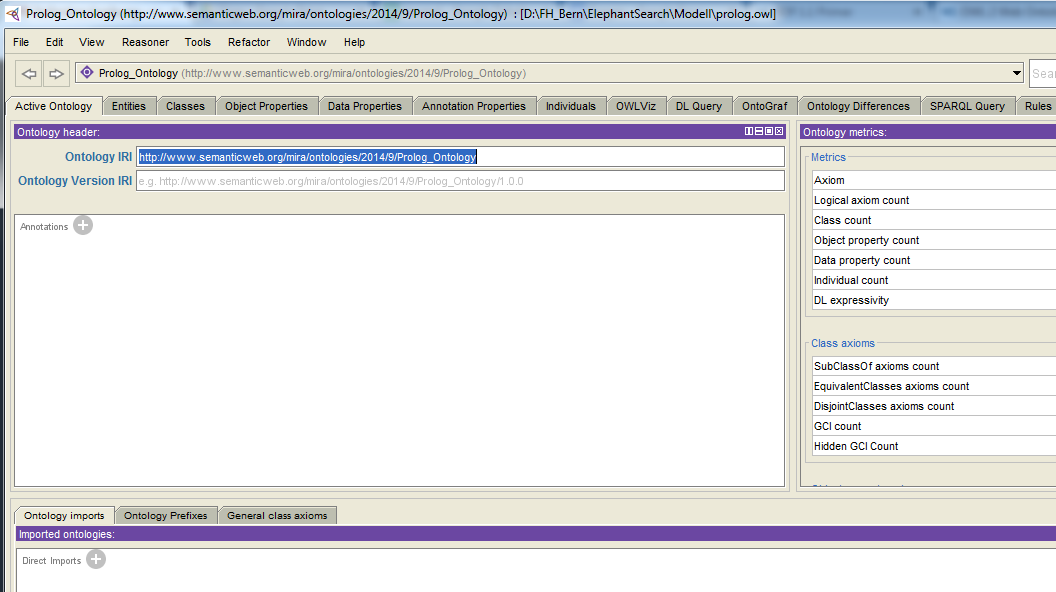
\includegraphics{bilder/protege.png}}}
\caption{Übersichtsfenster des Protégé-Editors\label{fig:protege}\protect\footnotemark}
\end{figure}
\footnotetext{Eigens erstellter Screenshot von Protégé}
\noindent\rule[1ex]{\textwidth}{1pt}
